\section*{\centering ПРИЛОЖЕНИЕ А}
\addcontentsline{toc}{section}{ПРИЛОЖЕНИЕ А}

\section*{Описание интерфейсов}

\begin{figure}[h]
	\centering
	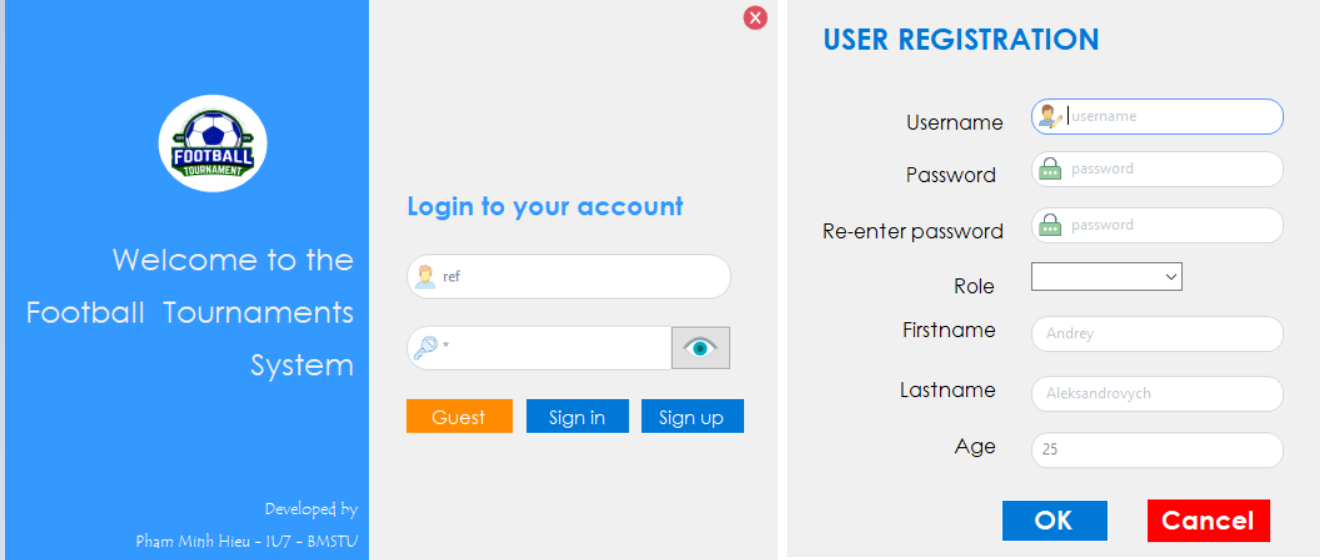
\includegraphics[height=0.25\textheight]{img/examples/demon1.png}
	\caption{Демонстрация работы программы при входе в систему и зарегистрации}
	\label{img:ex1}
\end{figure}

\begin{figure}[h]
	\centering
	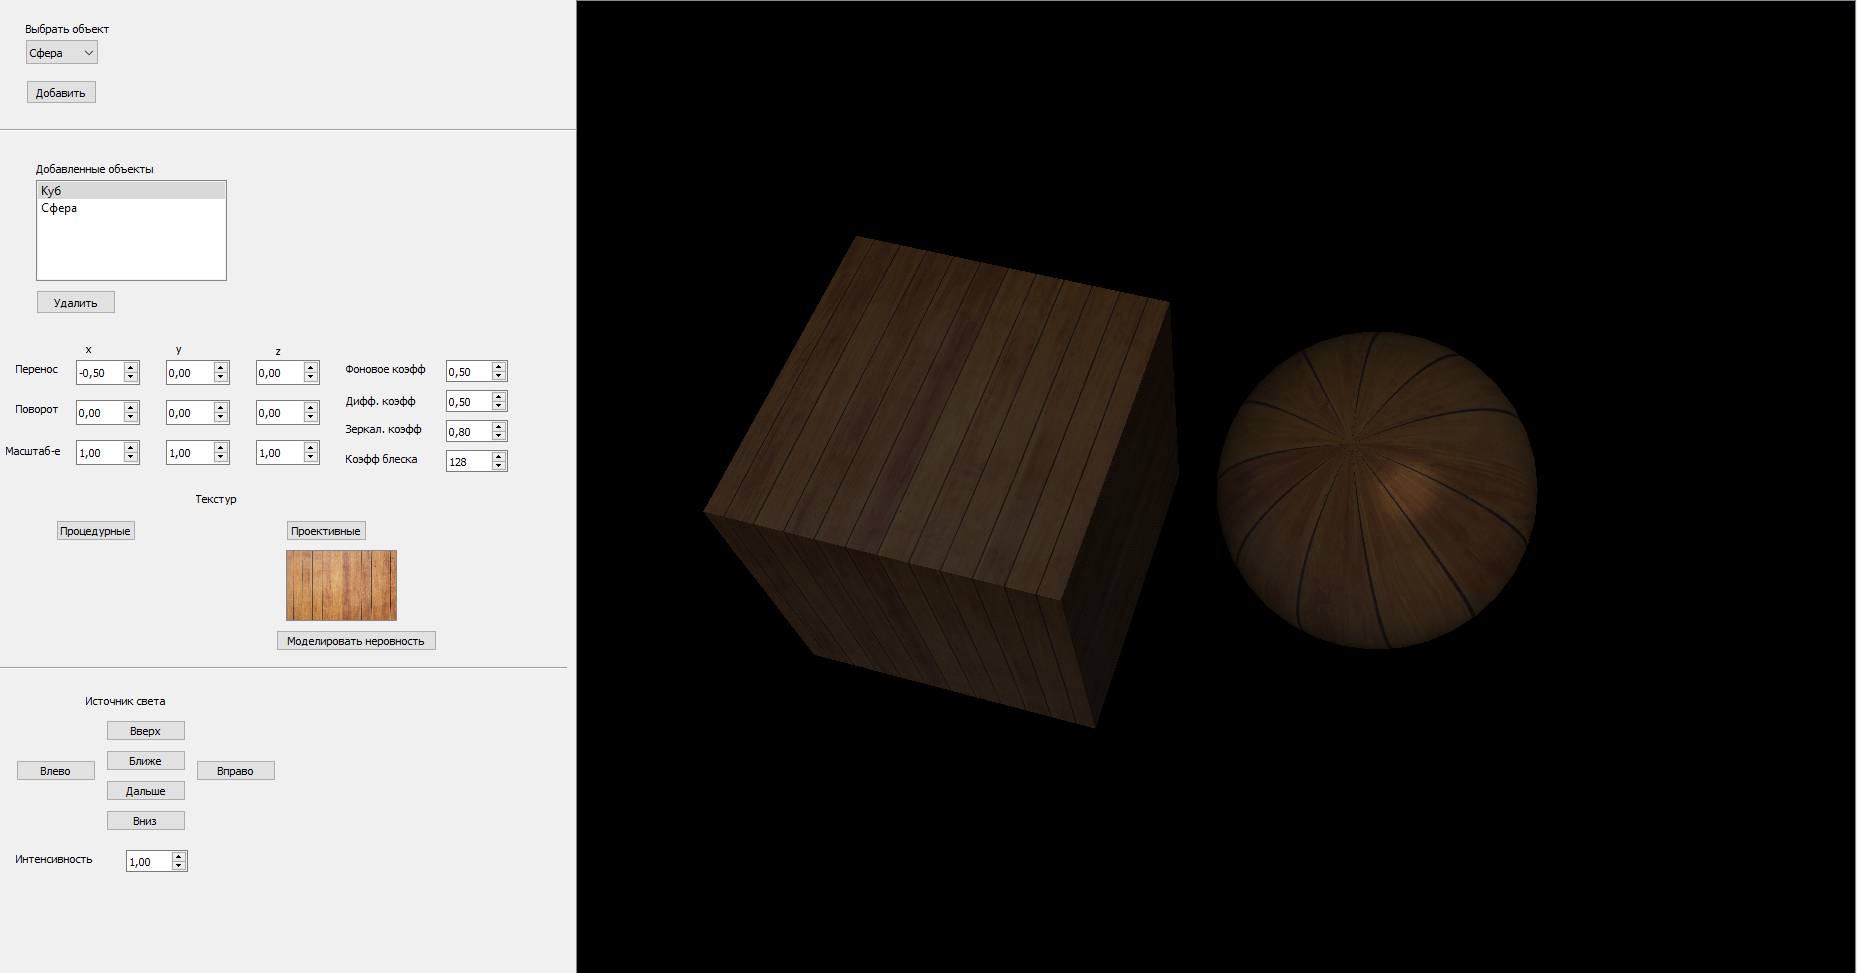
\includegraphics[height=0.3\textheight]{img/examples/demon2.png}
	\caption{Демонстрация главного экрана}
	\label{img:ex2}
\end{figure}
\clearpage
На рисунках \ref{img:ex4}--\ref{img:ex3} приведены демонстрации работы программы.
\begin{figure}[h]
	\centering
	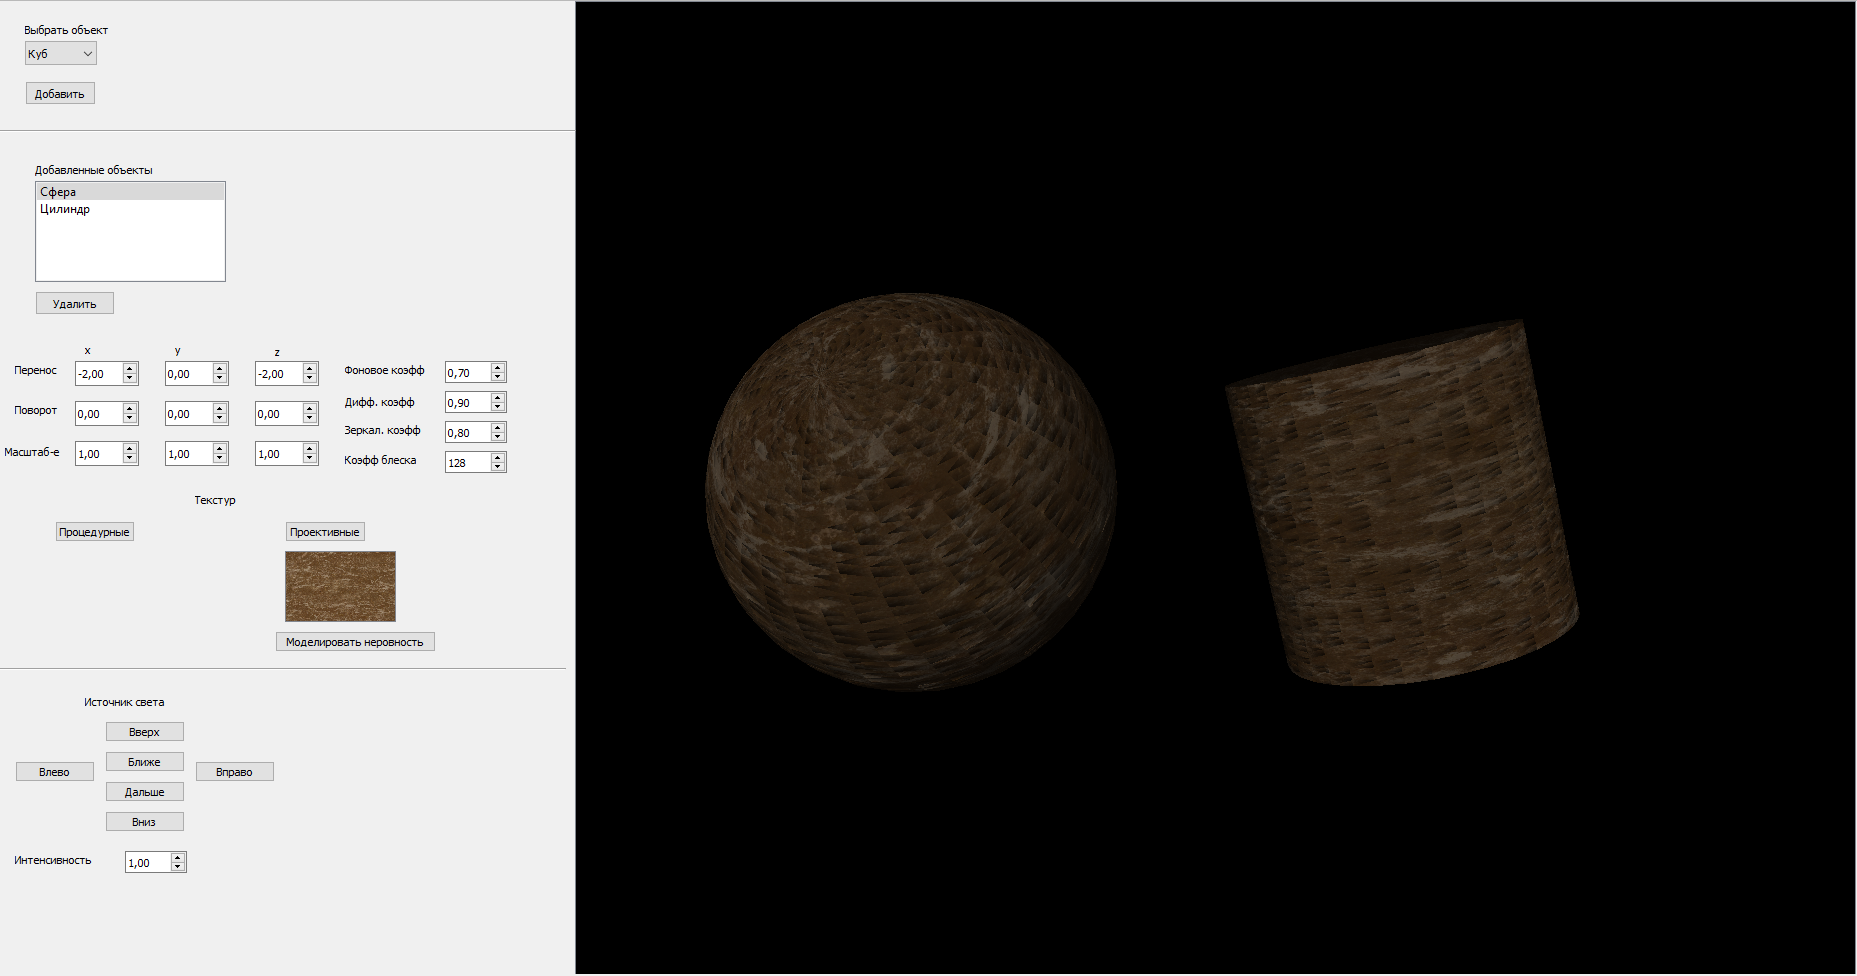
\includegraphics[height=0.3\textheight]{img/examples/demon3.png}
	\caption{Демонстрация работы программы при просмотре статистики турнира}
	\label{img:ex4}
\end{figure}

\begin{figure}[h]
	\centering
	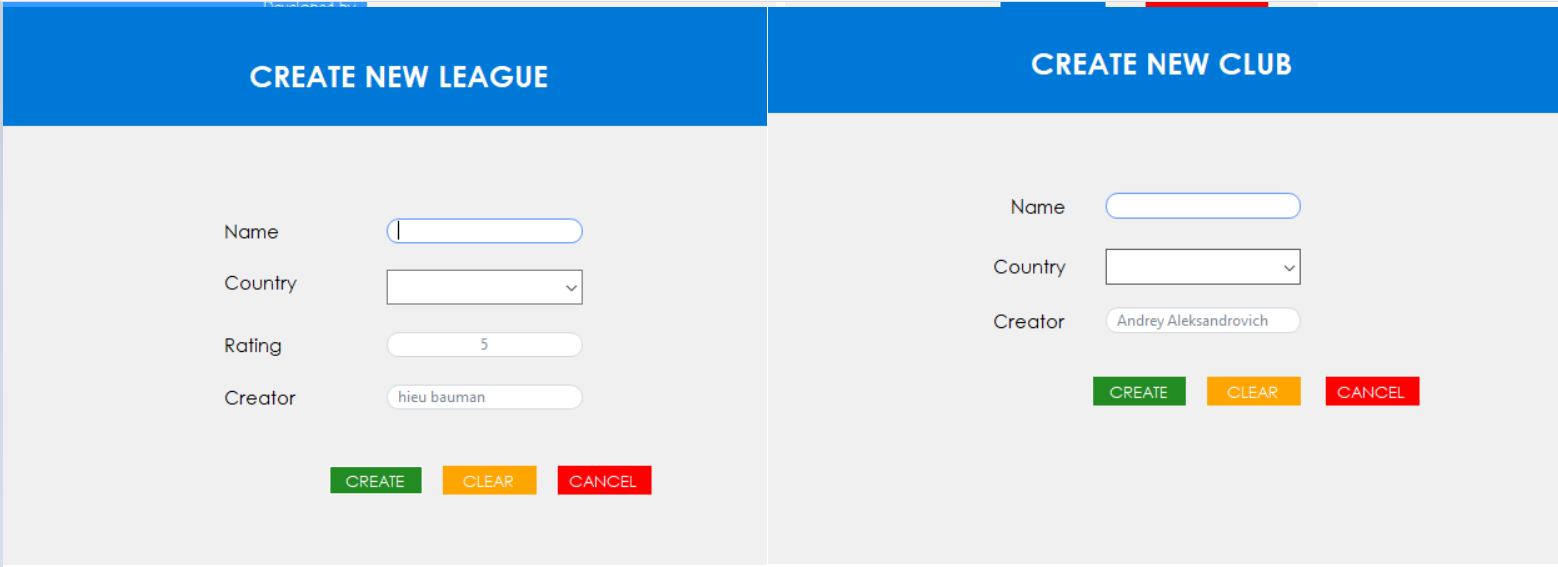
\includegraphics[height=0.2\textheight]{img/examples/demon4.png}
	\caption{Демонстрация работы программы при создании нового турнира и нового клуба}
	\label{img:ex3}
\end{figure}

\clearpage
На рисунках \ref{img:ex5}--\ref{img:ex6} приведены демонстрации работы программы.
\begin{figure}[h]
	\centering
	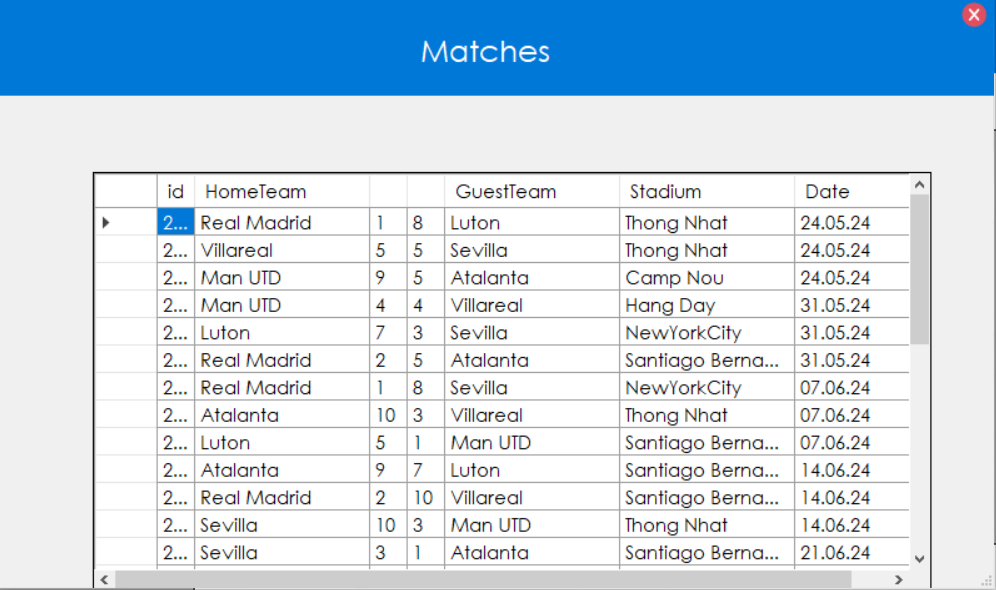
\includegraphics[height=0.3\textheight]{img/examples/demon5.png}
	\caption{Демонстрация работы программы при просмотре результата матчей}
	\label{img:ex5}
\end{figure}

\begin{figure}[h]
	\centering
	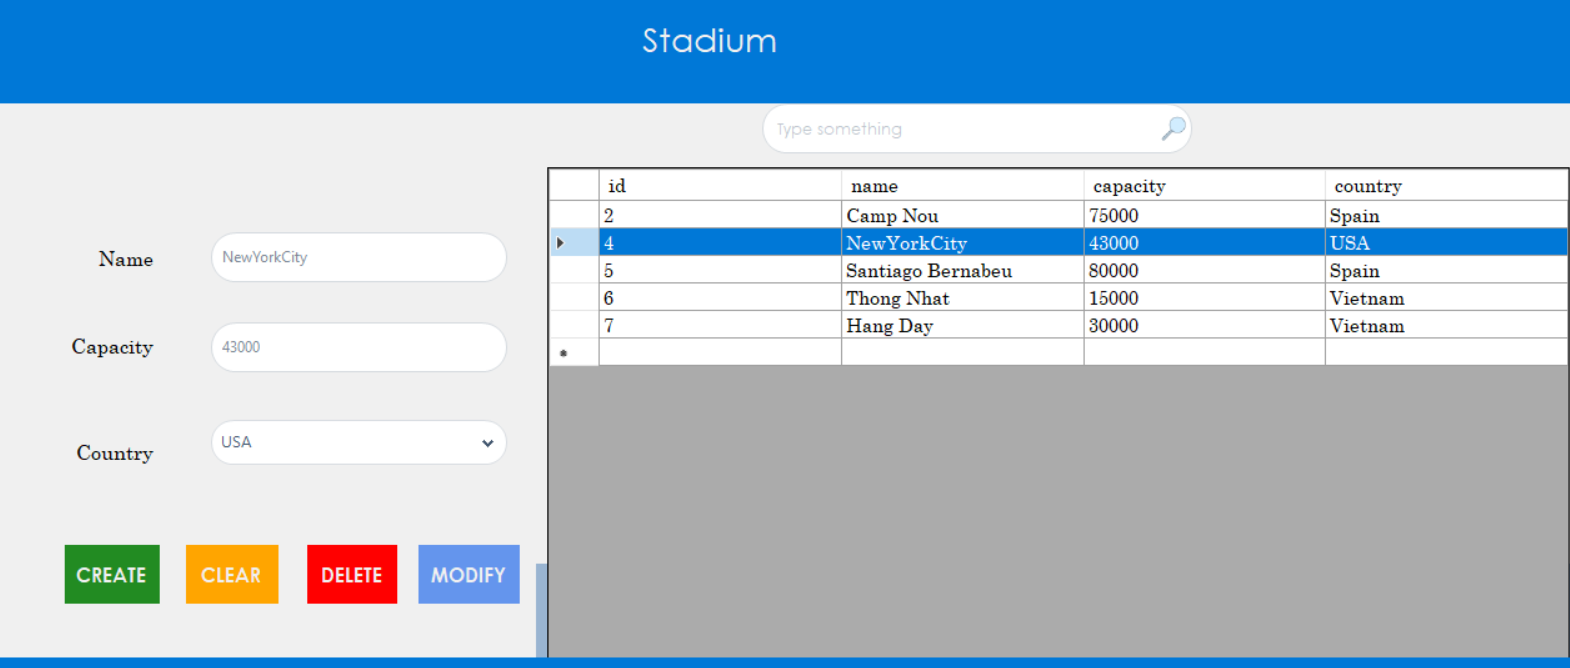
\includegraphics[height=0.25\textheight]{img/examples/demon6.png}
	\caption{Демонстрация работы программы при просмотре список стадионов}
	\label{img:ex6}
\end{figure}
\clearpage
\section*{Создание базы данных}
\begin{lstlisting}[caption={Создание всех таблиц}, label={lst:createtable}]
create table if not exists Users
(
	id serial primary key,
	login varchar(30) not null unique,
	password varchar(30) not null,
	role varchar(20) not null,
	firstname varchar(30) default 'hieu',
	lastname varchar(30) default 'bich',
	age int default 25,
	id_club int default -1,
);

create table if not exists Countries
(
	id serial not null primary key,
	name varchar(40) not null,
	continent varchar(40) not null
);

create table if not exists Clubs
(
	id serial not null primary key,
	name varchar(50) not null,
	id_country int not null,
	
	foreign key (id_country) references Countries(id) on delete cascade
);

create table if not exists Stadiums
(
	id serial not null primary key,
	name varchar(30) not null,
	capacity int not null,
	id_country int not null,
	
	foreign key (id_country) references Countries(id) on delete cascade
);

create table if not exists Leagues
(
	id serial not null primary key,
	name varchar(30) not null,
	rating float,
	id_user int,
	
	foreign key (id_user) references Users(id) on delete cascade
);

create table if not exists Matches
(
	id serial not null primary key,
	goal_home_club int not null,
	goal_guess_club int not null,
	id_league int not null,
	id_stadium int not null,
	id_home_club int not null,
	id_guess_club int not null,
	
	foreign key (id_league) references Leagues(id) on delete cascade,
	foreign key (id_stadium) references Stadiums(id) on delete cascade,
	foreign key (id_home_club) references Clubs(id) on delete cascade,
	foreign key (id_guess_club) references Clubs(id) on delete cascade
);

create table if not exists Requests
(
	id serial not null primary key,
	created_time timestamp default now(),
	id_league int default -1,
	id_club int not null,
	id_user int not null,
	
	foreign key (id_club) references Clubs(id) on delete cascade,
	foreign key (id_user) references Users(id) on delete cascade
);

create table if not exists Feedbacks
(
	id serial not null primary key,
	grade int not null,
	id_user int not null,
	id_league int not null,
	
	foreign key (id_user) references Users(id) on delete cascade,
	foreign key (id_league) references Leagues(id) on delete cascade
);

create table if not exists LeagueClub
(
	id serial not null primary key,
	id_league int not null,
	id_club int not null,
	
	foreign key (id_league) references Leagues(id) on delete cascade,
	foreign key (id_club) references Clubs(id) on delete cascade
);
\end{lstlisting}


\begin{lstlisting}[caption={Функция составляет турнирное расписание}, label={lst:f1}]
create or replace function create_schedule(id_l int) returns void as $$
declare
	size int;
	ss int;
	start_first_leg date := '2024-05-24';
	start_second_leg date;
	full_id int[];
	id_stadiums int[];
	week int;
	random_index int;
begin
	select array_agg(id_club) into full_id 
	from leagueclub where id_league = id_l;
	size := array_length(full_id, 1);
	select array_agg(id) into id_stadiums from stadiums;
	ss := array_length(id_stadiums, 1);
	
	start_second_leg := start_first_leg + INTERVAL '7' DAY * (size - 1);
	
	for week in 1..(size - 1) loop
		call createMatch(id_l, id_stadiums[getRandomNum(ss)], full_id[1], full_id[2], week, start_first_leg);
		
		call createMatch(id_l, id_stadiums[getRandomNum(ss)], full_id[2], full_id[1], week + size - 1, start_second_leg);
	
		for i in 0..(size / 2 - 2) loop
			call createMatch(id_l, id_stadiums[getRandomNum(ss)], full_id[3 + i], 
			full_id[size - i], week, start_first_leg);
			call createMatch(id_l, 
			id_stadiums[getRandomNum(ss)],
			 full_id[size - i], full_id[3 + i], 
			 week + size - 1, start_second_leg);			
		end loop;
		
		
		full_id = rotate_teams(full_id);
		start_first_leg := start_first_leg +
		 INTERVAL '7' day;
		start_second_leg := start_second_leg
		 + INTERVAL '7' day;
	end loop;
end;
$$
language plpgsql;

create or replace function rotate_teams(full_id int[])
returns int[] 
as
$$
declare
	last_id int;
	size int;
begin
	size := array_length(full_id, 1);
	last_id := full_id[size];
	
	for i in reverse size..3 loop
	full_id[i] := full_id[i - 1];
	end loop;
	
	full_id[2] := last_id;
	return full_id;
end;
$$
language plpgsql;
\end{lstlisting}

\begin{lstlisting}[caption={Реализация триггера}, label={lst:trigger}]
create or replace function calculate_rating()
returns trigger
as
$$
begin
	update leagues set rating = (select sum(f.grade) / count(*)::double precision as rating
	from feedbacks f
	where id_league = new.id_league)
	where id = new.id_league;
	
	return new;
end;
$$
language plpgsql;

create trigger auto_cal_rating
after insert on feedbacks
for each row execute function calculate_rating();
\end{lstlisting}

\begin{lstlisting}[caption={Создание роли администратора и выдыча права}, label={lst:role1}]
create role league_admin with
connection limit -1
login
password '#admin123';


grant all privileges
on all tables in schema public
to league_admin;
\end{lstlisting}

\begin{lstlisting}[caption={Создание роли судьи и выдыча права}, label={lst:role2}]
create role league_referee with
connection limit - 1
login
password '#referee123';

grant select on all tables in schema public
to league_referee;

grant insert on
public."leagues",
public."leagueclub",
public."feedbacks",
public."matches"
to league_referee;	

grant update on
public."leagues",
public."users",
public."matches"
to league_referee;

grant delete on
public."requests"
to league_referee;
\end{lstlisting}

\begin{lstlisting}[caption={Создание роли тренера и выдыча права}, label={lst:role3}]
create role league_coach with
connection limit - 1
login
password '#coach123';

grant select on all tables in schema public
to league_coach;

grant insert on
public."clubs",
public."feedbacks",
public."requests"
to league_coach;

grant update on
public."clubs",
public."users"
to league_coach;

grant delete on
public."requests"
to league_coach;

\end{lstlisting}

\begin{lstlisting}[caption={Создание роли футболиста и выдыча права}, label={lst:role4}]
create role league_footballer with
connection limit -1
login
password '#footballer123';

grant select on all tables in schema public
to league_footballer;

grant insert on
public."feedbacks",
public."requests"
to league_footballer;

grant update on
public."users"
to league_footballer;

grant delete on
public."requests",
public."feedbacks"
to league_footballer;
\end{lstlisting}

\begin{lstlisting}[caption={Создание роли гости и выдыча права}, label={lst:role5}]
create role league_guest with
connection limit -1
login
password '#guest123';

grant select on all tables in schema public
to league_referee;	

grant insert on
public."users",
public."feedbacks"
to league_guest
\end{lstlisting}

\begin{lstlisting}[caption={Реализация тестирования для функции get\_table\_league}, label={lst:test1}]
create or replace function test_get_table()
returns void as
$$
begin
	drop table if exists expected_res;
	create temp table if not exists expected_res
	(
	name varchar(64),
	allgames int,
	games int,
	wins int,
	draws int,
	loses int,
	goals int,
	losts int,
	diff int,
	points int
	);
	
	insert into expected_res values
	('Atalanta',	10,	10,	6,	0,	4,	59,	44,	15,	18),
	('Sevilla',	10,	10,	5,	3,	2,	56,	42,	14,	18),
	('Luton',	10,	10,	5,	1,	4,	67,	54,	13,	16),
	('Villareal',	10,	10,	4,	2,	4,	50,	48,	2,	14),
	('Real Madrid',	10,	10,	4,	1,	5,	38,	55,	-17,	13),
	('Man UTD',	10,	10,	1,	3,	6,	42,	69,	-27,	6);
	
	call auto_compare(5);
	
	truncate expected_res;
	insert into expected_res values
	('Atalanta',	6,	4,	2,	1,	1,	22,	21,	1,	7),
	('Villareal',	6,	3,	2,	0,	1,	25,	20,	5,	6),
	('Sevilla',	6,	3,	1,	1,	1,	18,	16,	2,	4),
	('Aston Villa',	6,	2,	0,	0,	2,	11,	19,	-8,	0);
	
	call auto_compare(4);
	
	truncate expected_res;
	insert into expected_res values
	('Arsenal',	6,	0,	0,	0,	0,	0,	0,	0,	0),
	('Aston Villa',	6,	0,	0,	0,	0,	0,	0,	0,	0),
	('Luton',	6,	0,	0,	0,	0,	0,	0,	0,	0),
	('Real Madrid',	6,	0,	0,	0,	0,	0,	0,	0,	0);
	
	call auto_compare(8);
	
	raise notice 'All tests passed';
end;
$$
language plpgsql;
\end{lstlisting}

\begin{lstlisting}[caption={Реализация тестирования для триггера auto\_cal\_rating}, label={lst:test2}]
CREATE OR REPLACE FUNCTION test_trigger()
RETURNS void AS $$
DECLARE
rec RECORD;
BEGIN
select rating from leagues where id in (5, 8, 9);
INSERT INTO feedbacks(grade, id_user, id_league) 
VALUES (3, 100, 5);
INSERT INTO feedbacks(grade, id_user, id_league) 
VALUES (5, 100, 8);
INSERT INTO feedbacks(grade, id_user, id_league) 
VALUES (1, 100, 9);


FOR rec IN (SELECT id, rating FROM leagues WHERE (id, rating) NOT IN ((5, 2.24), (8, 3), (9, 1))) LOOP
RAISE EXCEPTION 'Test failed: Unexpected result %', rec;
END LOOP;

RAISE NOTICE 'All tests passed';
END;
$$ LANGUAGE plpgsql;
\end{lstlisting}